\PassOptionsToPackage{unicode}{hyperref}
\PassOptionsToPackage{hyphens}{url}
%
\documentclass[12pt, a4paper]{article}
% NOTE: the course page requires 3cm margins (the original template had 1in)
\usepackage[a4paper,margin=3cm]{geometry}
\setlength\parindent{0pt}
\usepackage{mathptmx}
\usepackage{amsmath,amssymb}
\usepackage[T1]{fontenc}
\usepackage[utf8]{inputenc}
\usepackage{textcomp}
\usepackage{booktabs}   % nicer tables
\usepackage{graphicx}   % figures
\usepackage{placeins}   % \FloatBarrier keeps floats in their section
\setlength\parskip{4pt}
\renewcommand{\topfraction}{0.85}
\renewcommand{\textfraction}{0.1}
\renewcommand{\floatpagefraction}{0.8}

\author{Name1 Surname1, Degree Programme, ID number (matricola)
\\Name2 Surname2, Degree Programme, ID number (matricola)
\\Name3 Surname3, Degree Programme, ID number (matricola)
\\Name4 Surname4, Degree Programme, ID number (matricola)
\\Name5 Surname5, Degree Programme, ID number (matricola)}
\date{}
\title{Formal Departments and Informal Communication:\\
A Network Analysis of E-mail in a European Research Institution}

\begin{document}
\maketitle

\section{Introduction}
\label{introduction}

This project uses social network analysis to study communication inside an
organisation. In particular, we analyse the e-mails exchanged among the members
of a European research institution.

An organisation can be described in two ways. The first is its official
structure: every person belongs to a department, and departments are the units
where work is organised. The second is how people really work together: whom
they talk to and exchange information with. These two do not always match,
because people often need to work with colleagues outside their own department.
E-mail data is a good way to observe the second structure: it is recorded
automatically, it covers the whole organisation, and, unlike a survey, it does
not depend on what people remember \cite{borgatti2018}.

The dataset we use was published together with studies on how networks grow
over time \cite{leskovec2007} and on algorithms that find groups in a network
\cite{yin2017}. The second study uses the department of each person to check
whether an algorithm finds the right groups. We use the same information for a
different goal: to compare the official departments with the way people
actually communicate.

\section{Problem and Motivation}
\label{problem-and-motivation}

The problem we study is whether the division of a research institution into
departments affects whom its members e-mail, and how much. This question is
interesting for two reasons. In theory, it checks whether the official borders
between departments are also borders for communication. In practice, it shows
where information moves easily and where it may get stuck: a department whose
members write only to each other can become isolated, while the few people who
connect different departments become very important, because information
between departments depends on them.

We split the problem into three research questions:
\begin{itemize}
  \item \textbf{RQ1:} What is the overall structure of the e-mail network, and
        do departments differ structurally?
  \item \textbf{RQ2:} Who are the central actors, and who bridges departments?
  \item \textbf{RQ3:} Are departments real boundaries of communication?
\end{itemize}

The main contributions of the project are:
\begin{itemize}
  \item a description of the structure of the whole institution and of its four
        largest departments, tested against random networks that keep the
        number of contacts of every member;
  \item a list of the most central members and of the people who connect
        different departments;
  \item a statistical test of whether people in the same department e-mail each
        other more, and a comparison between the groups found from the e-mails
        and the official departments.
\end{itemize}

\section{Datasets}
\label{datasets}

% TODO (Person 2)
How did you gather the data? Did you digitise it? How? Is the material
publicly available? What tools did you use 1) to handle (store,
manipulate) the data and 2) to compute measures on the data?

\section{Validity and Reliability}
\label{validity}

\textbf{Validity.} We use e-mail as a proxy for working relationships, and
this proxy has four limits. First, an edge only records that at least one
e-mail was sent, so a single message, such as a reply to an announcement,
counts as much as daily collaboration; some edges are therefore not real
working relationships (errors of commission) \cite{borgatti2018}. Second, the
data only covers e-mails among members of the institution: e-mails with
outsiders, meetings, phone calls and chat are missing (errors of omission).
So 19 members (1.9\%) appear as isolated nodes, although they probably
communicate in other ways. Third, the data is anonymised, so we cannot check
members' roles, and the static version we use has no timestamps (a timestamped
version exists; see Section~\ref{critique}). Fourth, we take the department labels as
given: each member belongs to exactly one of 42 departments, even if some
people may work for two units, and 7 departments have fewer than five
members, which makes their measures unstable. The network is therefore a
valid picture of \emph{who} e-mails \emph{whom} inside the institution, but a
weaker picture of how strongly people work together.

\textbf{Reliability.} The study can be repeated exactly. The data is public
(Section~\ref{datasets}) and all networks were built with the same code and
rules, published in our GitHub repository
(github.com/foadas/network-analysis-email-eu). As an independent
check, our whole network has 24{,}929 directed edges after removing
self-loops, the same number of static edges that SNAP reports for the
timestamped version of the dataset. Every random procedure (baselines, permutations, Louvain,
rewiring) uses seeds derived from 42; re-running the full RQ3 notebook reproduced
every value of the first run exactly. Measures were computed in Python with
NetworkX 3.7, NMI and ARI with scikit-learn, and permutations with NumPy.

\section{Measures and Results}
\label{measures}

% ------------------------------------------------------------------
\subsection{Network structure (RQ1)}
\label{sec:structure}
% ------------------------------------------------------------------

To answer RQ1 we describe the whole network and compare it with the four
largest departments (IDs 4, 14, 1 and 21), each analysed as the network of
e-mails among its own members (Table~\ref{tab:structure}). We test two
hypotheses against 20 rewired networks that keep every member's degree.
\textbf{H1.1:} the network is small-world, i.e.\ more clustered than the rewired
networks with similar path lengths (H0: clustering is explained by the number of
contacts alone). \textbf{H1.2:} links are reciprocated more often than in- and
out-degrees explain (H0: reciprocity is explained by degrees alone). Clustering
and distances use the undirected (OR) network, in which two members are linked
if at least one e-mailed the other, and distances only its largest connected
component (LCC), because unconnected members have no distance.

\textbf{Density and reciprocity.} Density, the share of possible
sender--receiver pairs that exist, is 0.025 in the whole network: a member
writes to about 25 colleagues on average. In the departments it is four to seven
times higher (0.099--0.180). A random group of members would have the density of
the whole network, so this is not a size effect: members write much more inside
their department (Section~\ref{sec:departments}). Reciprocity, the share of
links that also exist in the opposite direction, is 0.68--0.82, against 0.13 in
the rewired whole network and 0.35--0.66 in the rewired departments; every
observed value is higher than all 20 rewired ones ($p=0.048$, the smallest value
possible with 20 networks). H1.2 is supported: links go both ways far more often
than activity levels explain, although in dense departments part of it is
expected (department~21: 0.82 against 0.66).

\textbf{Connectivity.} Ignoring direction, 98.1\% of the members are in one
connected component. Following direction, the largest strongly connected
component (SCC) holds 79.9\%, and its members are on average 2.55 e-mail steps
apart; 19 members (1.9\%) send and receive no e-mail, and the others can reach
the SCC or be reached from it, but not both. Departments~1 and~21 are less
connected: only 58.5\% and 52.5\% of their members are in the department SCC.
Of the 15 members of department~21 outside its LCC, 10 write only to other
departments and 5 send no e-mail; in department~1, 3 form a small separate
group, 3 write only outside and 3 send no e-mail.

\textbf{Small-world structure (H1.1).} The average clustering coefficient $C$ is
the probability that two contacts of a member are also linked; the average
shortest path length $L$ is the mean number of steps between two members
\cite{newman2018}. In the whole network $C=0.407$ and $L=2.59$ (diameter 7),
against $C=0.162$ and $L=2.44$ in the rewired networks: clustering is 2.5 times
higher than in all 20 of them ($z=92$, $p=0.048$), while paths are only 6\%
longer, so $\sigma=(C/C_{null})/(L/L_{null})=2.4$, above the small-world
threshold of 1 \cite{watts1998,humphries2008}. H1.1 is supported: members form
close groups, yet two connected members are less than three steps apart.
Transitivity, the share of closed triangles, is lower (0.267) than $C$,
probably because the contacts of the most active members are less often linked
to each other.

Departments~4, 14 and~21 are also more clustered than chance (by 23\%, 15\% and
6\%; $p=0.048$) with paths at most 3\% longer ($\sigma$ 1.04--1.20).
Department~1 is not: its clustering is what its degrees alone produce ($z=0.4$,
$p=0.33$) and its paths are 27\% longer ($\sigma=0.80$). The coefficient
$\omega$ \cite{telesford2011} (0 for a small world, negative for lattice-like,
positive for random-like networks) agrees: it is close to 0 in all departments
($-0.11$ to $+0.06$), with department~1 the most lattice-like. So the
departments differ: department~1 is a looser network with longer chains, and
departments~1 and~21 are the least connected.

\textbf{Triad census.} To see which local patterns create the clustering, we
counted the 16 possible configurations of links among three members
\cite{borgatti2018} and compared them with directed rewired networks. In the
whole network, triangles of three mutual links (type 300) are 38 times more
frequent than expected and two mutual links sharing a member (201) 13 times,
while transitive triads (030T), which suggest a hierarchy, and cycles (030C) are
14 and 50 times rarer, and a member writing to two colleagues who do not write
to each other (021D) six times rarer (all $|z|>60$). Departments show the same
pattern, more weakly. Clustering thus comes from groups of colleagues who all
write to each other, not from chains of command; this partly reflects the high
reciprocity, which the null model does not keep.

\textbf{Degree distribution.} Figure~\ref{fig:degree} shows the cumulative
in-degree (colleagues a member hears from) and out-degree (colleagues a member
writes to) of the whole network. Both have a long tail: the median member writes
to 14 colleagues and hears from 17, while 4.3\% write to and 3.0\% hear from 100
or more (at most 333 and 211). These members are candidates for the central
roles in Section~\ref{sec:centrality}. The curve bends downward instead of
following a straight line, and with about 1{,}000 nodes a power-law fit would
not be reliable \cite{newman2018}, so we do not claim that the network is
scale-free.

\begin{table}[htbp]
\centering
\small
\begin{tabular}{lrrrrr}
\toprule
 & Whole & Dept 4 & Dept 14 & Dept 1 & Dept 21 \\
\midrule
Nodes                         & 1005  & 109   & 92    & 65    & 61    \\
Edges (directed)              & 24929 & 1167  & 1506  & 502   & 601   \\
Density                       & 0.025 & 0.099 & 0.180 & 0.121 & 0.164 \\
Reciprocity                   & 0.711 & 0.723 & 0.708 & 0.681 & 0.819 \\
Reciprocity, deg.-pres.\ null  & 0.131 & 0.354 & 0.378 & 0.495 & 0.655 \\
Mean in/out degree            & 24.80 & 10.71 & 16.37 & 7.72  & 9.85  \\
LCC share of nodes            & 0.981 & 0.927 & 0.967 & 0.862 & 0.754 \\
Largest SCC share             & 0.799 & 0.789 & 0.859 & 0.585 & 0.525 \\
Transitivity                  & 0.267 & 0.424 & 0.457 & 0.545 & 0.665 \\
Avg.\ clustering $C$          & 0.407 & 0.471 & 0.520 & 0.587 & 0.660 \\
Avg.\ clustering, deg.-pres.\ null & 0.162 & 0.381 & 0.453 & 0.581 & 0.622 \\
Avg.\ shortest path $L$       & 2.587 & 2.165 & 1.830 & 2.450 & 1.788 \\
Avg.\ shortest path, deg.-pres.\ null & 2.440 & 2.105 & 1.829 & 1.936 & 1.757 \\
Directed avg.\ shortest path (SCC) & 2.547 & 2.190 & 1.856 & 1.810 & 1.448 \\
Diameter                      & 7     & 5     & 4     & 5     & 4     \\
$\sigma$ (vs deg.-pres.\ null)  & 2.37  & 1.20  & 1.15  & 0.80  & 1.04  \\
$\omega$                      & --    & $0.063$ & $0.063$ & $-0.106$ & $-0.014$ \\
\bottomrule
\end{tabular}
\caption{Structural measures of the whole network and of the four largest
departments. Density, reciprocity, SCC share and directed path length use the
directed network;
transitivity uses the whole undirected (OR) network; average clustering, path
lengths, diameter, $\sigma$ and $\omega$ use the undirected largest connected
component. ``Deg.-pres.\ null'': mean of 20 rewired networks keeping every
member's degree (in- and out-degree for reciprocity). $\omega$ was not computed
for the whole network because of its computing time.}
\label{tab:structure}
\end{table}

\begin{figure}[htbp]
\centering
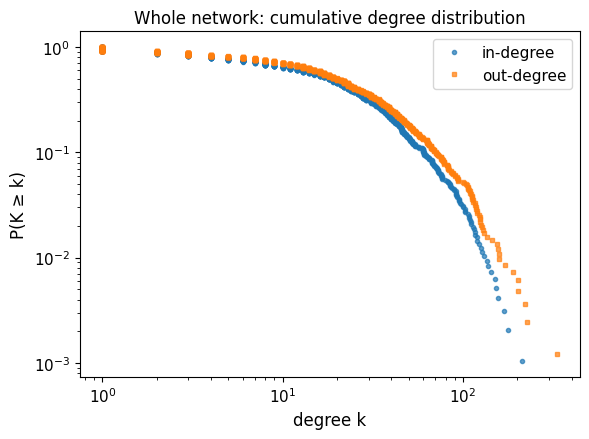
\includegraphics[width=0.7\textwidth]{degree_ccdf.png}
\caption{Cumulative in- and out-degree distributions $P(K\ge k)$ of the whole
network on log-log axes (members with degree 0 not shown). The long tail shows a
few members with more than 100 contacts.}
\label{fig:degree}
\end{figure}

\FloatBarrier

% ------------------------------------------------------------------
\subsection{Central actors and bridges (RQ2)}
\label{sec:centrality}
% TODO (Person 2)

% ------------------------------------------------------------------
\subsection{Departments as communication boundaries (RQ3)}
\label{sec:departments}

To answer RQ3 we test four hypotheses. In each, H0 is that department
membership and e-mailing are unrelated (for H3.3: that the e-mail communities and
the departments are unrelated). \textbf{H3.1:} members e-mail their own
department more than chance. \textbf{H3.2:} departments are more closed than
chance, but to different degrees. \textbf{H3.3:} the groups found from the
e-mails match the departments. \textbf{H3.4:} links across departments are less
often reciprocated. The null models are shuffled department labels,
degree-preserving rewired networks and shuffled communities
(Table~\ref{tab:rq3}). A last, descriptive analysis looks at pairs of
departments.

\textbf{H3.1: members prefer their own department.} If departments are
boundaries, most e-mails should stay inside them. About one edge in three
(34.7\%) joins two members of the same department, while only one in twenty
(4.7\%) would if e-mails ignored departments. Two colleagues
from the same department are about eleven times more likely to be connected
than two from different departments. The assortativity coefficient
\cite{newman2003}, which is 0 when people mix at random, confirms this with a
value of 0.31. Because e-mail links are not independent, we did not use a
$\chi^2$ test but the Quadratic Assignment Procedure (QAP) \cite{krackhardt1988}:
it correlates the e-mail matrix with a matrix that marks
same-department pairs, then shuffles the departments 5{,}000 times. No shuffle
came close to the observed correlation, so the preference is significant
($p=0.0002$). The boundary is not closed, however: two thirds of all edges
still cross departments.

\textbf{H3.2: some departments are much more closed than others.} Next we asked
\emph{which} departments are closed. The E--I index \cite{krackhardtstern1988} compares a department's
external and internal edges in the undirected network: it is $-1$ if all edges stay inside and $+1$ if
all go outside. Small departments have few possible partners, so we compare
each department with its value under 5{,}000 random relabellings. Of the 35 departments with at least five members, 34 are
significantly more closed than this baseline (Benjamini--Hochberg adjusted
$p<0.05$ \cite{benjamini1995}).
Department~14 is the only one with more internal than external edges and
behaves like a silo; departments~17 and~7 come close. The exception is
department~31: its 8 members have no edge among themselves (E--I $=1.00$), but
with so few members even random e-mailing would give almost no internal edges,
so the test cannot show a boundary either way. The other departments closest to
random mixing are also small (5 to 13 members). Among departments with at least 20 members,
the most open are 23, 6 and~36, with an E--I of about 0.90 against 0.97--0.98
expected; in departments~23 and~6, 8 and 11 members write to no one in their
own department.

\textbf{H3.3: e-mail groups join departments together.} If departments were
the real units of communication, a method that sees only the e-mails should
rediscover them. With the standard resolution and seed 42, the Louvain method
\cite{blondel2008} finds 9 communities (7 to 9 over 20 seeds) plus the 19
isolated members, with a modularity much higher than in rewired networks with
the same degrees. The 42 departments, used as groups, reach 70\% of this
modularity. Figure~\ref{fig:communities} shows that 86\% of the members are in
the main community of their department, but most communities join several
departments (the largest joins 27); only C7 and C8, mostly made of the two most
closed departments (14 and 17), are almost a single department. We measure the agreement between communities and departments with
normalised mutual information (NMI) and the adjusted Rand index (ARI)
\cite{danon2005,hubert1985}, which are about 0 for unrelated partitions and 1
for identical ones. The agreement is moderate: NMI 0.60 and ARI 0.36 for seed
42, one of the best of 20 seeds (medians 0.58 and 0.31), but far above shuffled
communities. At resolution 3, Louvain finds 42 communities, as many as the
departments, and the agreement only rises to NMI 0.73 and ARI 0.59: at the
standard resolution communities combine departments, and even at the
departments' own scale they only partly match them.

\textbf{Department pairs (descriptive).} Counting the edges
between departments, three quarters of the pairs (641 of 861) exchange some e-mail, but
half of all cross-department edges fall in only 61 pairs. These busy pairs
often share a Louvain community (both departments have most members in it): 41\%
of the 61 busiest pairs do, twice the 22\% of all connected pairs, and so do 7
of the 10 busiest pairs without department~36, such as departments~4 and~5 or~21
and~22. This is consistent with communities merging departments that e-mail
each other intensely. Department~36 does not fit this pattern: with 2\% of the members, it takes part in 23\% of all
cross-department edges and writes to 40 of the 41 other departments, like a
service unit for the whole institution (see Section~\ref{sec:centrality}).

\textbf{H3.4: links across departments are less often two-way.} Finally, a
boundary can change the kind of communication, not only its amount. Splitting
the reciprocity of Section~\ref{sec:structure}, 75\% of links inside
departments are reciprocated (the other member has also written at least once),
against 69\% across departments. The difference is
larger than in all 5{,}000 shuffles ($p=0.0002$): contact between departments is
more often one-way.

\begin{table}[htbp]
\centering
\small
\begin{tabular}{llrrrr}
\toprule
 & Measure & Observed & Null mean & $p$ & 20 seeds \\
\midrule
H3.1 & Assortativity by department          & 0.314 & $-0.002$ & 0.0002 & -- \\
H3.1 & QAP correlation $r$                  & 0.226 & 0.000    & 0.0002 & -- \\
H3.3 & Modularity $Q$, Louvain              & 0.413 & 0.122    & 0.0099 & 0.40--0.42 \\
H3.3 & Modularity $Q$, departments          & 0.288 & $-0.004$ & 0.0099 & -- \\
H3.3 & NMI, communities vs departments      & 0.596 & 0.062    & 0.0010 & 0.53--0.60 \\
H3.3 & ARI, communities vs departments      & 0.355 & 0        & --     & 0.24--0.36 \\
H3.4 & Reciprocity within / between         & 0.752 / 0.689 & --  & 0.0002 & -- \\
\bottomrule
\end{tabular}
\caption{Tests for RQ3. Null models: 5{,}000 permutations of department labels
(H3.1, H3.4), 100 degree-preserving rewired networks ($Q$), 1{,}000 shuffled
community assignments (NMI); the ARI null mean is 0 by construction. Louvain:
resolution 1; Observed = seed 42; last column: seeds 42--61. One-sided
$p$-values; 0.0002, 0.0099 and 0.0010 are the smallest values these numbers of
permutations allow. H3.1 and H3.4 use the directed edges, $Q$ the undirected
(OR) edges.}
\label{tab:rq3}
\end{table}

\begin{figure}[htbp]
\centering
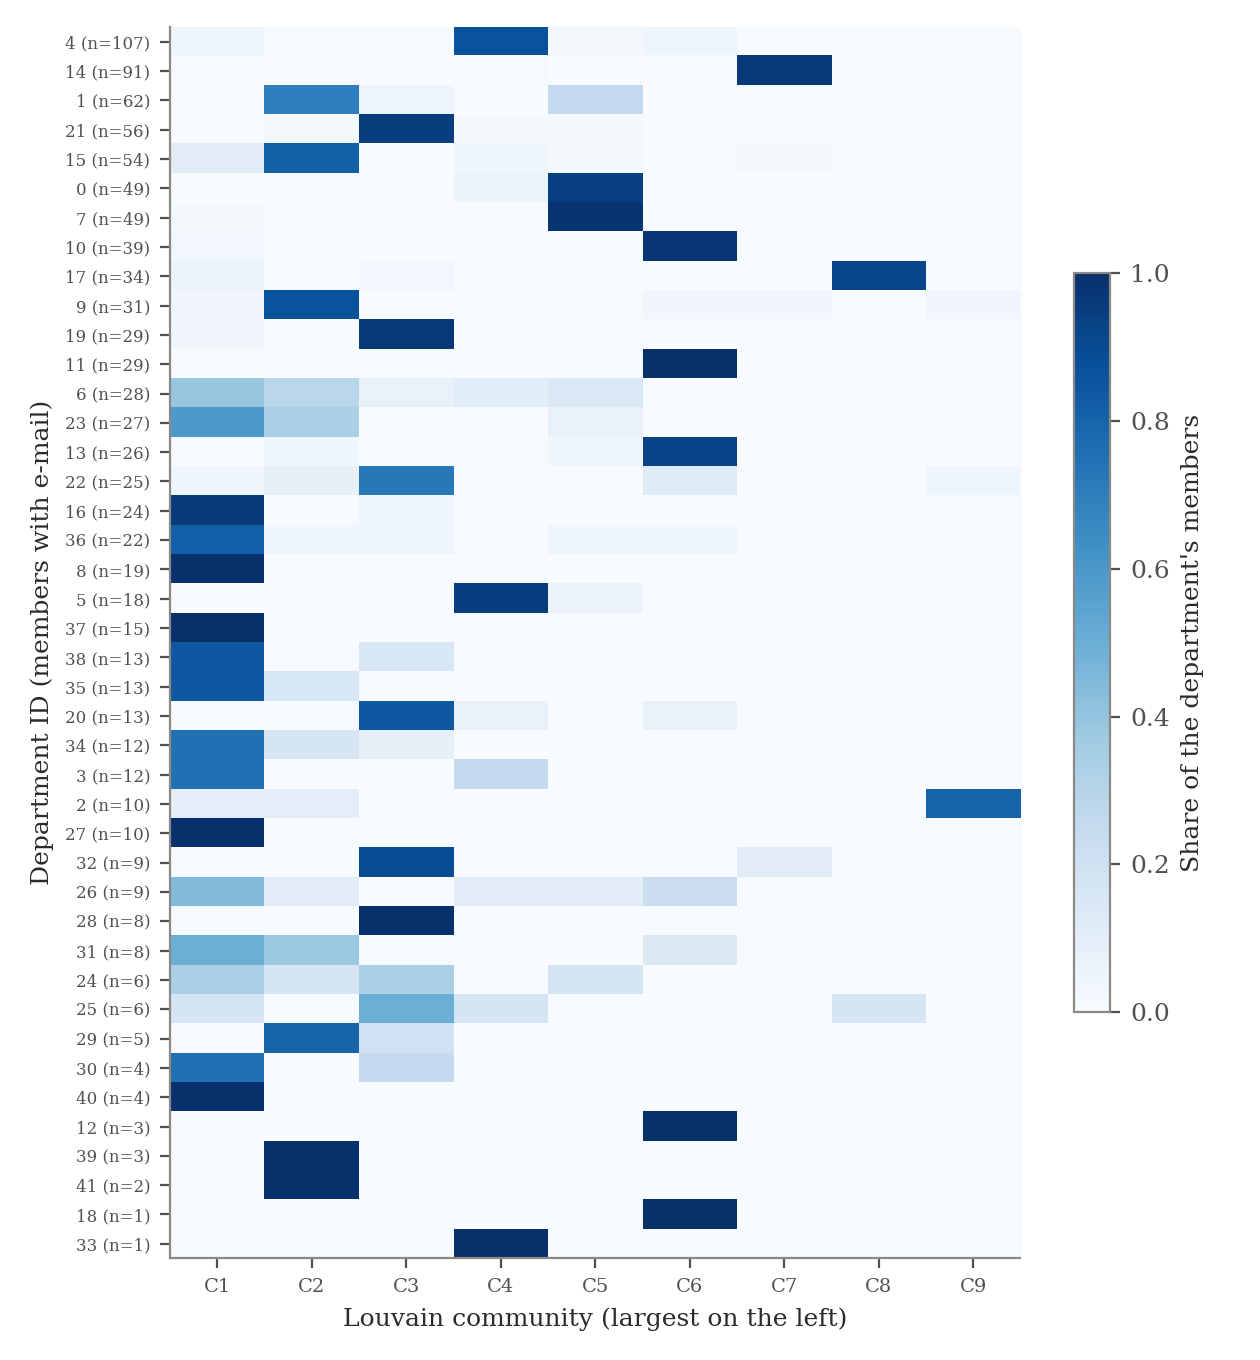
\includegraphics[width=0.62\textwidth]{fig_5_3_departments_vs_communities.png}
\caption{Share of each department's members (rows) in each Louvain community
(columns), isolated members excluded. Most rows have one dark cell (departments
stay together), but many columns have several (communities merge
departments).}
\label{fig:communities}
\end{figure}



\section{Conclusion}
\label{conclusion}

\subsection{RQ1: network structure}
The e-mail network is a small-world network: clustering is far higher than in
random networks with the same degrees, while, ignoring direction, two connected
members are less than three steps apart, and links are reciprocated far more
often than activity levels explain (H1.1, H1.2). Following direction, paths
inside the core are as short (2.55 steps), but a fifth of the members are
outside the core, so information can spread quickly among most, but not all,
members. Locally, it consists of groups of colleagues who all write to each
other, not of hierarchies. Departments~4, 14 and~21 share this
structure, while department~1 has clustering at chance level and longer paths;
departments~1 and~21 are also the least connected, with only about half of their
members able to reach each other by following e-mails.

% TODO 6.2 (Person 2)

\subsection{RQ3: departments as boundaries}
Departments are real but permeable boundaries of communication. A member is
about eleven times more likely to e-mail a colleague of the same department,
34 of the 35 tested departments are more closed than chance, and links
inside departments are more often two-way. Yet two thirds of the e-mail links
cross departments, and the groups that emerge from the e-mails only partly
match the departments: at the standard resolution they keep most departments
together but merge them into a few larger blocks, often along the department
pairs that e-mail each other most. Closure also varies: department~14 works
almost as a silo, while mid-sized departments such as 6 and~23 are the least
closed.

\subsection{Overall}
Departments clearly shape whom members e-mail, but they do not contain
communication. The institution forms one small world in which departments are
dense, mostly reciprocal clusters (RQ1, RQ3); yet two thirds of the links cross
departments, concentrated in a few department pairs and in department~36, which
works as a hub for the whole institution.
% TODO (Person 2): one sentence linking the central members and bridges of RQ2.
The formal structure therefore explains a large part, but not all, of the
informal one.


\section{Critique}
\label{critique}

\subsection{RQ1: network structure}
This part has three limits. First, the network only records whether two
people exchanged at least one e-mail over the whole period: one message counts
as much as daily contact, and a short path may not be possible in time order.
The timestamped version of the dataset would allow a weighted and temporal
analysis. Second, the rewired null models keep each member's number of contacts
but nothing else, and $\omega$ could not be computed for the whole network,
because building its lattice reference takes too long. Third, the department
networks are small (61--109 members) and keep only internal e-mails, so their
results are less certain.

% TODO 7.2 (Person 2)

\subsection{RQ3: departments as boundaries}
Four limits apply. First, Louvain is randomised: the exact communities and
their match with the departments vary between seeds (ARI 0.24--0.36), and the
number of communities depends on the resolution; we checked resolutions from
0.5 to 3 and the match stays partial. Modularity can also miss small groups
\cite{fortunato2007}, so another method could draw different groups. Second, many departments are small: their E--I index is uncertain,
seven departments were not tested, and NMI and ARI ignore the 19 isolated
members. Third, QAP shows that sharing a department is associated with
e-mailing, not why: colleagues may also share an office or a project, which
the data does not record. Finally, all results come from a single
institution.


\begin{thebibliography}{99}
\bibitem{benjamini1995} Y.~Benjamini, Y.~Hochberg. Controlling the false
  discovery rate: a practical and powerful approach to multiple testing.
  \emph{Journal of the Royal Statistical Society B}, 57(1):289--300, 1995.
\bibitem{blondel2008} V.~D. Blondel, J.-L. Guillaume, R.~Lambiotte,
  E.~Lefebvre. Fast unfolding of communities in large networks. \emph{Journal
  of Statistical Mechanics}, P10008, 2008.
\bibitem{borgatti2018} S.~P. Borgatti, M.~G. Everett, J.~C. Johnson.
  \emph{Analyzing Social Networks}. 2nd ed., Sage, 2018.
\bibitem{danon2005} L.~Danon, A.~D\'{\i}az-Guilera, J.~Duch, A.~Arenas. Comparing
  community structure identification. \emph{Journal of Statistical Mechanics},
  P09008, 2005.
\bibitem{fortunato2007} S.~Fortunato, M.~Barth\'elemy. Resolution limit in
  community detection. \emph{PNAS}, 104(1):36--41, 2007.
\bibitem{humphries2008} M.~D. Humphries, K.~Gurney. Network `small-world-ness':
  a quantitative method for determining canonical network equivalence.
  \emph{PLoS ONE}, 3(4):e0002002, 2008.
\bibitem{hubert1985} L.~Hubert, P.~Arabie. Comparing partitions. \emph{Journal
  of Classification}, 2:193--218, 1985.
\bibitem{krackhardt1988} D.~Krackhardt. Predicting with networks:
  nonparametric multiple regression analysis of dyadic data. \emph{Social
  Networks}, 10(4):359--381, 1988.
\bibitem{krackhardtstern1988} D.~Krackhardt, R.~N. Stern. Informal networks and
  organizational crises: an experimental simulation. \emph{Social Psychology
  Quarterly}, 51(2):123--140, 1988.
\bibitem{leskovec2007} J.~Leskovec, J.~Kleinberg, C.~Faloutsos. Graph evolution:
  densification and shrinking diameters. \emph{ACM Transactions on Knowledge
  Discovery from Data}, 1(1), 2007.
\bibitem{newman2003} M.~E.~J. Newman. Mixing patterns in networks.
  \emph{Physical Review E}, 67:026126, 2003.
\bibitem{newman2018} M.~Newman. \emph{Networks}. 2nd ed., Oxford University Press, 2018.
\bibitem{telesford2011} Q.~K. Telesford, K.~E. Joyce, S.~Hayasaka,
  J.~H. Burdette, P.~J. Laurienti. The ubiquity of small-world networks.
  \emph{Brain Connectivity}, 1(5):367--375, 2011.
\bibitem{watts1998} D.~J. Watts, S.~H. Strogatz. Collective dynamics of
  `small-world' networks. \emph{Nature}, 393:440--442, 1998.
\bibitem{yin2017} H.~Yin, A.~R. Benson, J.~Leskovec, D.~F. Gleich. Local
  higher-order graph clustering. In \emph{Proceedings of the 23rd ACM SIGKDD
  International Conference on Knowledge Discovery and Data Mining}, 2017.
\end{thebibliography}

\end{document}
